%======================================================================
\section{Processamento: detecção de queda}\label{sec:queda}
%======================================================================
Esta seção resume o relatório do Q1~\cite{q1}, que desenvolveu e comparou os modelos no
computador, e descreve a versão que roda na pulseira.

\subsection{Por que um modelo}

O primeiro detector da pulseira era um limiar: queda quando $\amag$ passa de 2,5\,g. Ele pega
as quedas, mas também correr, pular, subir escada depressa e sentar com força. Na base
pública SisFall, com o sensor na faixa da pulseira, esse limiar deu \textbf{69,9 alarmes falsos
por hora} de atividade (a métrica está na Seção~\ref{sec:metrica}). O que separa uma queda de uma corrida não é o tamanho do pico, e sim
o que vem antes e depois dele: a queda livre ($\amag$ abaixo de 1\,g) logo antes do impacto e,
depois, o corpo parado em outra posição (Figura~\ref{fig:janela}).

\subsection{Dados}

\begin{itemize}
  \item \textbf{SisFall}~\cite{sisfall}: \sisPessoas{} pessoas (23 jovens e 15 idosos), 4505
        ensaios a 200\,Hz, com o sensor na cintura: \adlEnsaios{} atividades de \adlTipos{} tipos
        (\adlHoras\,h) e \quedasEnsaios{} quedas de 15 tipos. Os sinais foram saturados em $\pm$8\,g para imitar a
        pulseira.
  \item \textbf{Nossos ensaios}: os 18 do primeiro semestre (Seção~\ref{sec:mpu}), na cintura e
        em $\pm$2\,g, usados só como teste.
\end{itemize}

\subsection{Pipeline}

Todos os métodos compartilham o mesmo pipeline, e é ele que roda na pulseira:
\begin{enumerate}
  \item \textbf{Filtro}: passa-baixa de 20\,Hz nos 6 eixos (Seção~\ref{sec:cond_digital}).
  \item \textbf{Gatilho}: um pico de $\amag$ filtrado de \gatilhoLon\,g ou mais, emitido depois de
        0,5\,s sem um valor maior. Ele deixa passar \gatilhoPassam\,\% das quedas e dispara
        $\sim$\gatilhoDisparosH{} vezes por hora de atividade: o gatilho só acorda o
        classificador (Figura~\ref{fig:pipeline}).
  \item \textbf{Janela}: de $-1{,}0$ a $+0{,}8$\,s em volta do pico.
  \item \textbf{Atributos}: \nAtributos{} medidas no tempo: estatísticas de $\amag$ e de
        $\wmag$, a queda livre antes do impacto, a quietude e a média de $\amag$ no fim da
        janela, a mudança de inclinação e a correlação entre os eixos.
  \item \textbf{Classificador}: decide queda ou não queda, com uma probabilidade.
\end{enumerate}

\begin{figure}[H]
\centering
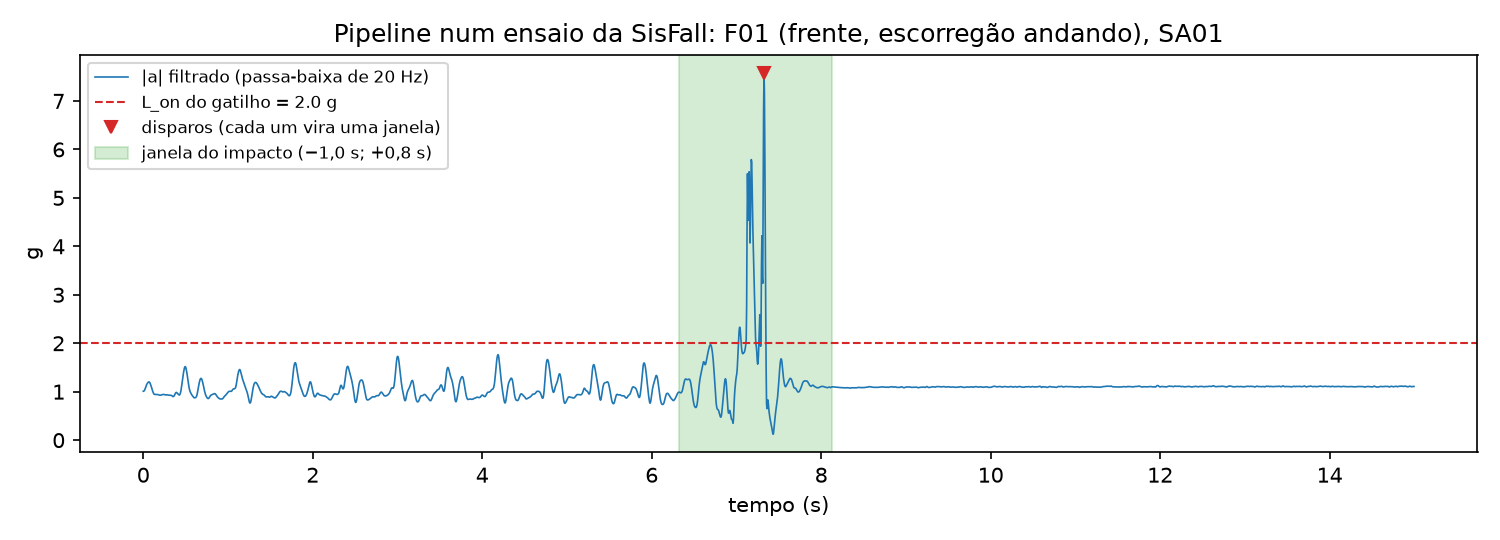
\includegraphics[width=\linewidth]{figuras/fig_pipeline.png}
\caption{O pipeline numa queda da SisFall: o sinal filtrado, o nível do gatilho e a janela
classificada em volta do impacto.}
\label{fig:pipeline}
\end{figure}

\begin{figure}[H]
\centering
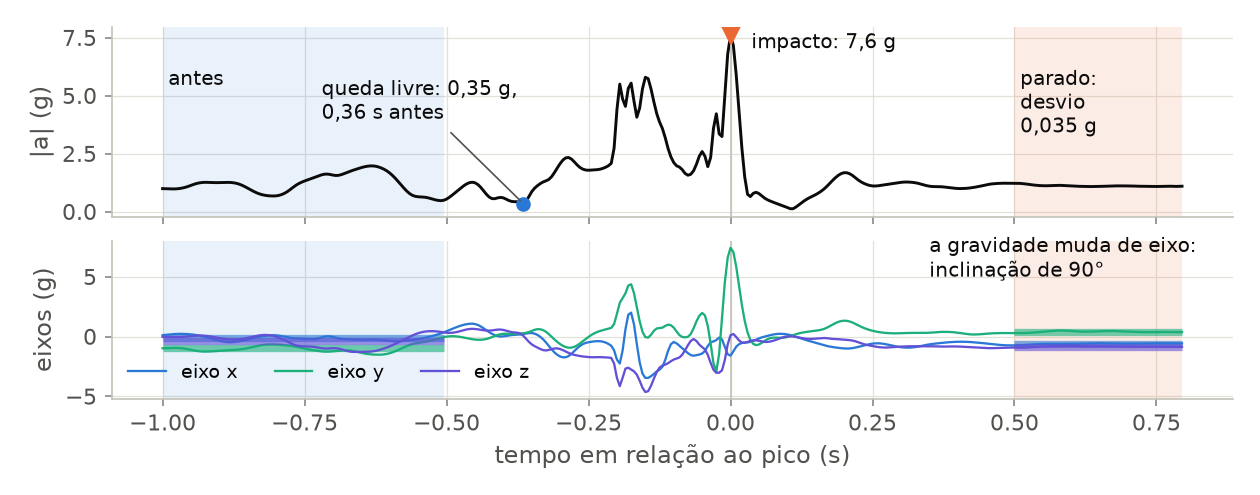
\includegraphics[width=\linewidth]{figuras/fig_janela.png}
\caption{A janela de uma queda e o que os atributos medem: a queda livre antes do impacto, o
impacto e o corpo parado em outra posição (a gravidade muda de eixo).}
\label{fig:janela}
\end{figure}

\subsection{A métrica: alarmes falsos por hora de atividade}\label{sec:metrica}

Um detector de queda erra de dois jeitos: deixa passar uma queda, ou chama o cuidador sem que
ninguém tenha caído. O primeiro erro se mede pela fração das quedas detectadas. O segundo, pelos
\textbf{alarmes falsos por hora de atividade}: quantas vezes o sistema chamaria o cuidador à toa
a cada hora em que o residente está se movimentando. As duas medidas andam juntas: baixar o
limiar pega mais quedas e dá mais alarmes, e subir faz o contrário.

\paragraph{Que horas são essas.} São as \adlHoras\,h de atividades da SisFall: os
\adlEnsaios{} ensaios sem queda, de \adlTipos{} tipos, feitos pelas \sisPessoas{} pessoas
(Tabela~\ref{tab:horas_atividade}). Cada tipo de ensaio tem uma duração prevista, de 100\,s
para andar e correr a 12\,s para os movimentos curtos, como sentar, deitar e agachar, e a soma
das durações de todos os ensaios é o denominador. São horas só de movimento, e de movimentos escolhidos para parecer queda: correr,
descer escada depressa, sentar de uma vez numa cadeira baixa, desabar na cadeira, tropeçar e
pular. Ficam de fora as horas paradas de um dia real, como dormir, comer e ver televisão, em
que o gatilho quase não dispara. Por isso, uma hora de atividade da SisFall gera mais alarmes
que uma hora qualquer do dia.

\begin{table}[H]
\centering
\caption{As horas de atividade da SisFall, o denominador da métrica.}
\label{tab:horas_atividade}
\small
% Gerado por modelo/experimentos/12_relatorio_q2.py a partir da SisFall (dados/publicos)
\begin{tabular}{@{}l l r r r r@{}}
\toprule
Atividades & Tipos & Ensaios & \makecell[r]{Cada ensaio\\(s)} & Horas & Parte \\
\midrule
Andar e correr & D01--D04 & 150 & 100 & 4,3 & 29\,\% \\
Subir e descer escada & D05--D06 & 308 & 25 & 2,1 & 15\,\% \\
Sentar e levantar da cadeira & D07--D11 & 940 & 12 & 3,1 & 22\,\% \\
Deitar e virar na cama & D12--D14 & 500 & 12 & 1,7 & 11\,\% \\
Agachar e curvar & D15--D16 & 380 & 12 & 1,3 & 9\,\% \\
Entrar e sair do carro & D17 & 189 & 25 & 1,3 & 9\,\% \\
Tropeçar e pular & D18--D19 & 240 & 12 & 0,8 & 5\,\% \\
\midrule
\textbf{Total} & 19 tipos & 2707 & & \textbf{14,5} & 100\,\% \\
\bottomrule
\end{tabular}

\end{table}

\paragraph{A conta.} Para o Random Forest da pulseira (Seção~\ref{sec:rf_pulseira}):
\begin{enumerate}
  \item Cada janela recebe a probabilidade dada por um modelo treinado sem a pessoa dela
        (validação cruzada por pessoa, em 5 dobras). Assim, o resultado vale para alguém que o
        modelo nunca viu.
  \item O gatilho abre \adlJanelas{} janelas nas atividades, \gatilhoDisparosH{} por hora, e
        \impactos{} janelas de impacto nas \quedasEnsaios{} quedas.
  \item O limiar é o que deixa 95\,\% das janelas de impacto acima dele: $P \ge \text{\rfLimiar}$.
  \item Com esse limiar, \rfAlarmesN{} das \adlJanelas{} janelas de atividade passam como
        queda. São os alarmes falsos:
        \[
          \frac{\text{\rfAlarmesN{} alarmes falsos}}{\text{\adlHoras\,h de atividade}}
          \approx \text{\rfAlarmes{} alarme falso por hora.}
        \]
  \item Nesse ponto, o modelo detecta \rfSensEnsaio\,\% das quedas. A conta é por queda, e não
        por janela: entram também as quedas que o gatilho perdeu, e por isso o número fica abaixo
        dos 95\,\%.
\end{enumerate}
A coluna ``Quedas com $\le$1 alarme/h'' da Tabela~\ref{tab:modelos_pulseira} faz a pergunta ao
contrário. Se o cuidador aceitar até um alarme falso por hora de atividade, ou seja,
\alarmesPermitidos{} nas \adlHoras\,h, o limiar pode descer até ficarem só
\alarmesPermitidos{} janelas de atividade acima dele. Quantas quedas passam então? Para o
Random Forest, \rfQuedas\,\%.

\paragraph{Por que essa métrica.}
\begin{itemize}
  \item \textbf{Mede o que custa na ILPI.} Cada alarme falso tira o cuidador de outro
        residente. Com alarmes demais, a equipe deixa de acreditar no sistema, e a queda de
        verdade também fica sem resposta. Contado por hora, o número vira alarmes por dia e por
        plantão: basta multiplicar pelas horas de atividade e pelo número de residentes.
  \item \textbf{Não engana como a acurácia.} Quase todas as janelas são de atividade, e um
        detector que nunca chama acerta quase todas elas. A especificidade por janela também
        engana. A do Random Forest é de \rfEspecJanela\,\%, o que parece perfeito, mas o número
        de alarmes depende de quantas janelas o gatilho abre: com o mesmo acerto por janela, um
        gatilho que abrisse dez vezes mais janelas daria dez vezes mais alarmes. Contados por
        hora, os alarmes já levam o gatilho em conta.
  \item \textbf{Compara métodos diferentes.} O AR, o DTW, a rede convolucional e os
        classificadores de atributos olham janelas de tamanhos diferentes, abertas em momentos
        diferentes. Dividir pelo tempo põe todos na mesma unidade.
  \item \textbf{Vem sempre com as quedas detectadas.} Zero alarme é fácil: basta nunca chamar.
        Por isso os métodos são comparados no mesmo ponto, o limiar que deixa 95\,\% das
        janelas de impacto acima dele, como num ponto da curva ROC.
  \item \textbf{Liga ao requisito.} O RNF08 pede no máximo um alarme falso por dia por
        residente (Tabela~\ref{tab:rnf}). Com \rfAlarmes{} alarme por hora de atividade, a conta
        fecha enquanto o residente tiver até \rnfHorasDia\,h por dia de movimento parecido com o
        da SisFall.
\end{itemize}

\paragraph{Limites.} A conta vale para os ensaios da SisFall: curtos, encenados em laboratório
e com o sensor na cintura. No pulso, o braço faz movimentos que a cintura não vê, como
gesticular e bater a mão na mesa, e eles também podem disparar o gatilho. A conversão para
alarmes por dia dá só a ordem de grandeza. A medida que vale é a do uso contínuo da pulseira,
prevista na verificação do RNF08.

\subsection{Comparação}

O Q1 comparou 22 métodos: os das aulas (modelos autorregressivos AR e ARX, correlação com
sinais de referência, DTW, atributos no tempo e em frequência, distâncias) e os usuais na
literatura (regras, regressão logística, árvore, SVM, Random Forest e redes convolucionais).
A avaliação é por pessoa: nenhuma pessoa aparece no treino e no teste ao mesmo tempo. A métrica
é a da Seção~\ref{sec:metrica}: alarmes falsos por hora de atividade, com cerca de 94\,\% das
quedas detectadas (Figura~\ref{fig:resumo}). O AR descreve bem a atividade normal, mas, usado como detector de
anomalia, dispara em qualquer movimento brusco; os métodos de atributos com um classificador
foram muito melhores.

\begin{figure}[H]
\centering
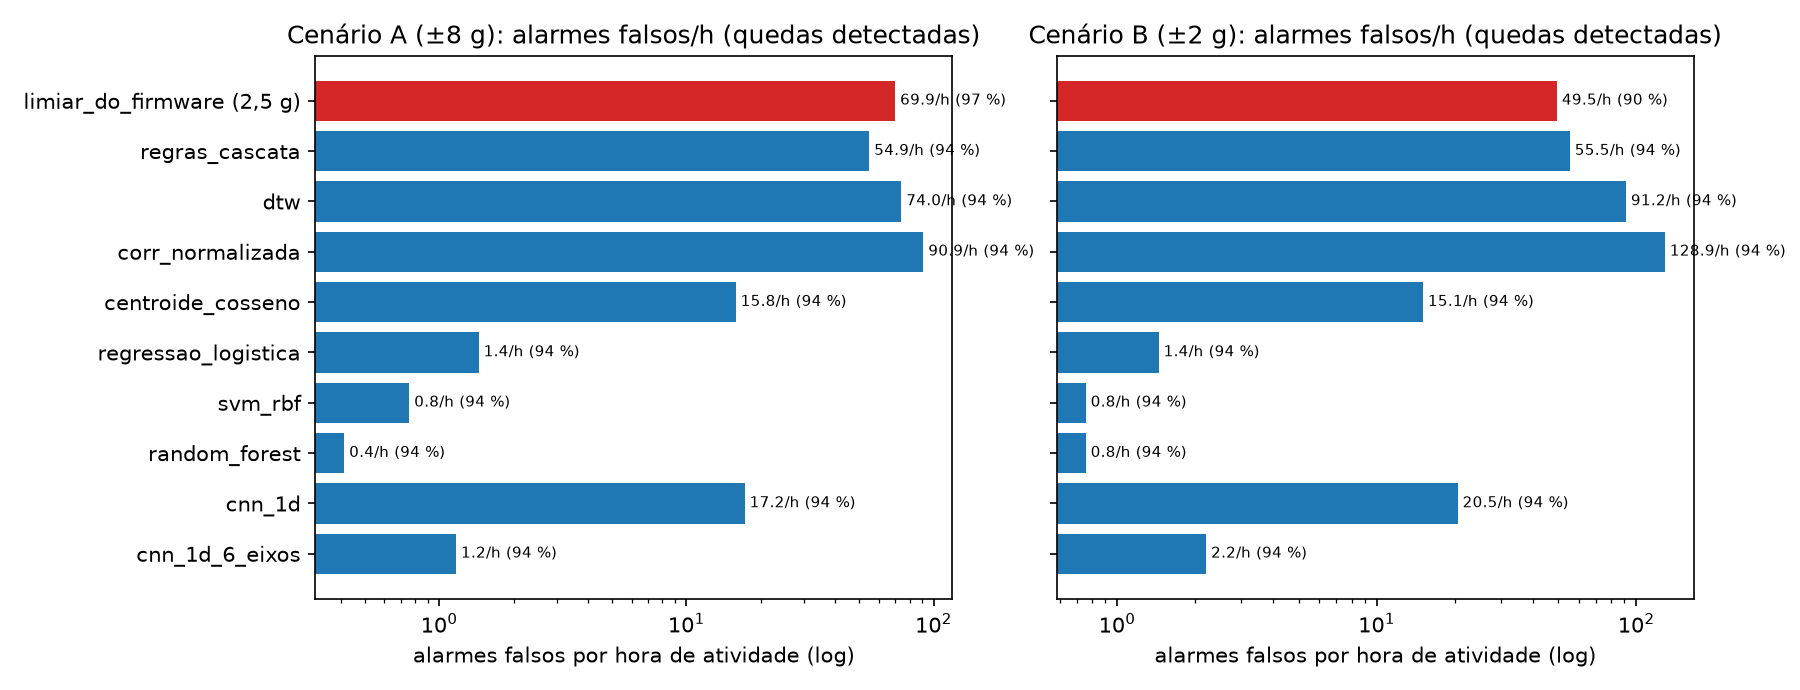
\includegraphics[width=\linewidth]{figuras/fig_resumo.png}
\caption{Alarmes falsos por hora de atividade de alguns dos métodos comparados no Q1, com a
fração de quedas detectadas entre parênteses. Cenário A: $\pm$8\,g, como a pulseira.}
\label{fig:resumo}
\end{figure}

\subsection{O modelo da pulseira}\label{sec:rf_pulseira}

Na configuração exata da pulseira (gatilho causal, os \nAtributos{} atributos no tempo,
$\pm$8\,g), três classificadores ficaram na disputa (Tabela~\ref{tab:modelos_pulseira}). As
diferenças entre eles cabem no erro da estimativa: os intervalos de 95\,\% das diferenças,
obtidos sorteando pessoas, passam pelo zero. O \textbf{Random Forest}~\cite{breiman} ficou: não precisa
padronizar os atributos, a probabilidade que vai no alerta é a fração de árvores que votaram
queda, e ele mostra quais atributos pesam (Figura~\ref{fig:importancia}). O SVM só entraria no
firmware se ganhasse com folga, porque exigiria outro classificador em C e outros testes.

\begin{table}[H]
\centering
\caption{Classificadores na configuração da pulseira (SisFall, validação por pessoa).}
\label{tab:modelos_pulseira}
\small
% Gerado por modelo/experimentos/12_relatorio_q2.py a partir de resultados/pulseira.json e svm_pulseira.json
\begin{tabular}{@{}lrrrr@{}}
\toprule
Classificador & \makecell[r]{Alarmes\\falsos/h} & \makecell[r]{Quedas com\\$\le$1 alarme/h} & \makecell[r]{Memória\\(kB)} & \makecell[r]{Operações\\por janela} \\
\midrule
Regressão logística & 0,62 & 94,9\,\% & 0,3 & 69 \\
Random Forest (60 árvores, prof. 10) & 0,55 & 95,1\,\% & 106,2 & 600 \\
SVM (RBF) & 0,69 & 96,2\,\% & 33,6 & 24\,012 \\
\bottomrule
\end{tabular}

\end{table}

\begin{figure}[H]
\centering
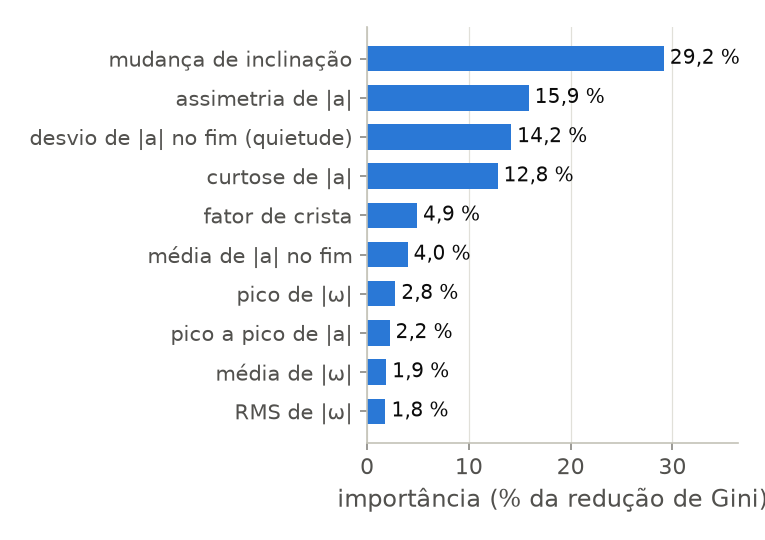
\includegraphics[width=0.9\linewidth]{figuras/fig_importancia.png}
\caption{Importância dos atributos no Random Forest da pulseira.}
\label{fig:importancia}
\end{figure}

O modelo tem 60 árvores de profundidade até 10 (\rfNos{} nós) e decide queda quando
$P \ge \text{\rfLimiar}$. No pipeline completo, sobre toda a SisFall, ele dá \rfAlarmes{} alarme falso
por hora de atividade e detecta \rfQuedas\,\% das quedas com no máximo um alarme falso por hora
(Figura~\ref{fig:funil}).

\begin{figure}[H]
\centering
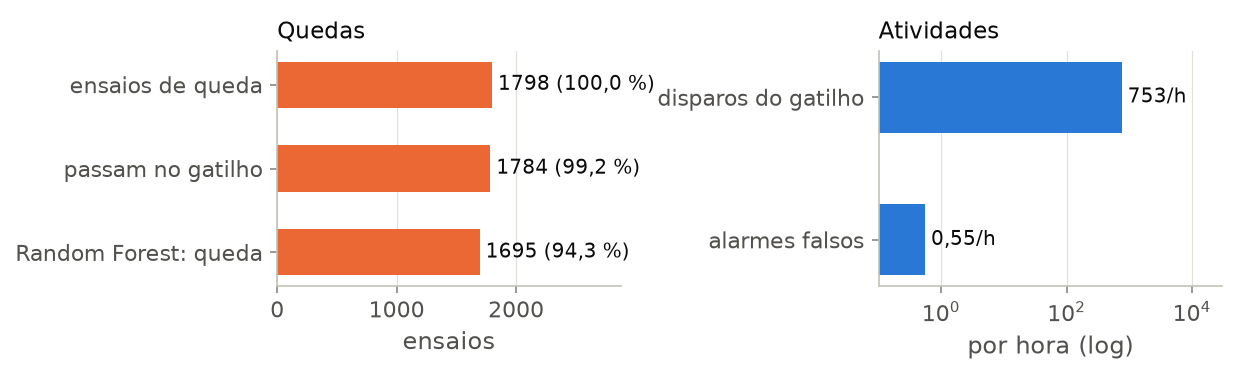
\includegraphics[width=\linewidth]{figuras/fig_funil_pulseira.png}
\caption{O pipeline da pulseira na SisFall: das quedas, quantas passam no gatilho e quantas o
Random Forest confirma; das atividades, quantos disparos e quantos alarmes falsos por hora.}
\label{fig:funil}
\end{figure}

\subsection{A versão embarcada}

O modelo vai para o firmware como código C gerado: um script Python exporta a floresta como
tabelas de nós (\rfBytes{} bytes de flash), os coeficientes do filtro, o gatilho e o limiar, e
gera junto os vetores de teste. O pipeline em C roda amostra a amostra na task
\code{sampling}, com o filtro do ESP-DSP e um buffer circular por eixo; a janela só é
classificada quando o gatilho dispara. O custo em ciclos de cada classificação é medido e vai
para o log.

A garantia de que o C faz o mesmo que o Python é o teste de paridade: em 26 janelas de 8
trechos da SisFall, o C acha os mesmos picos, calcula os atributos dentro da tolerância e dá
a mesma probabilidade, até $10^{-6}$ (885 verificações, Tabela~\ref{tab:testes}). Na placa, o
modo de coleta permite a mesma comparação com o sinal real do sensor: ele manda o sinal bruto
e cada janela classificada pela serial, para o Python refazer as contas.

\subsection{Nos nossos ensaios e limitações}

Nos 18 ensaios do primeiro semestre, o Random Forest treinado só na SisFall não deu nenhum
alarme ao andar ou correr e pegou as quedas de frente e de costas, mas perdeu as três quedas de
joelhos (Figura~\ref{fig:proprios}). São poucos ensaios, de uma pessoa só, mas o tipo de
queda que falhou fica marcado para a coleta.

\begin{figure}[H]
\centering
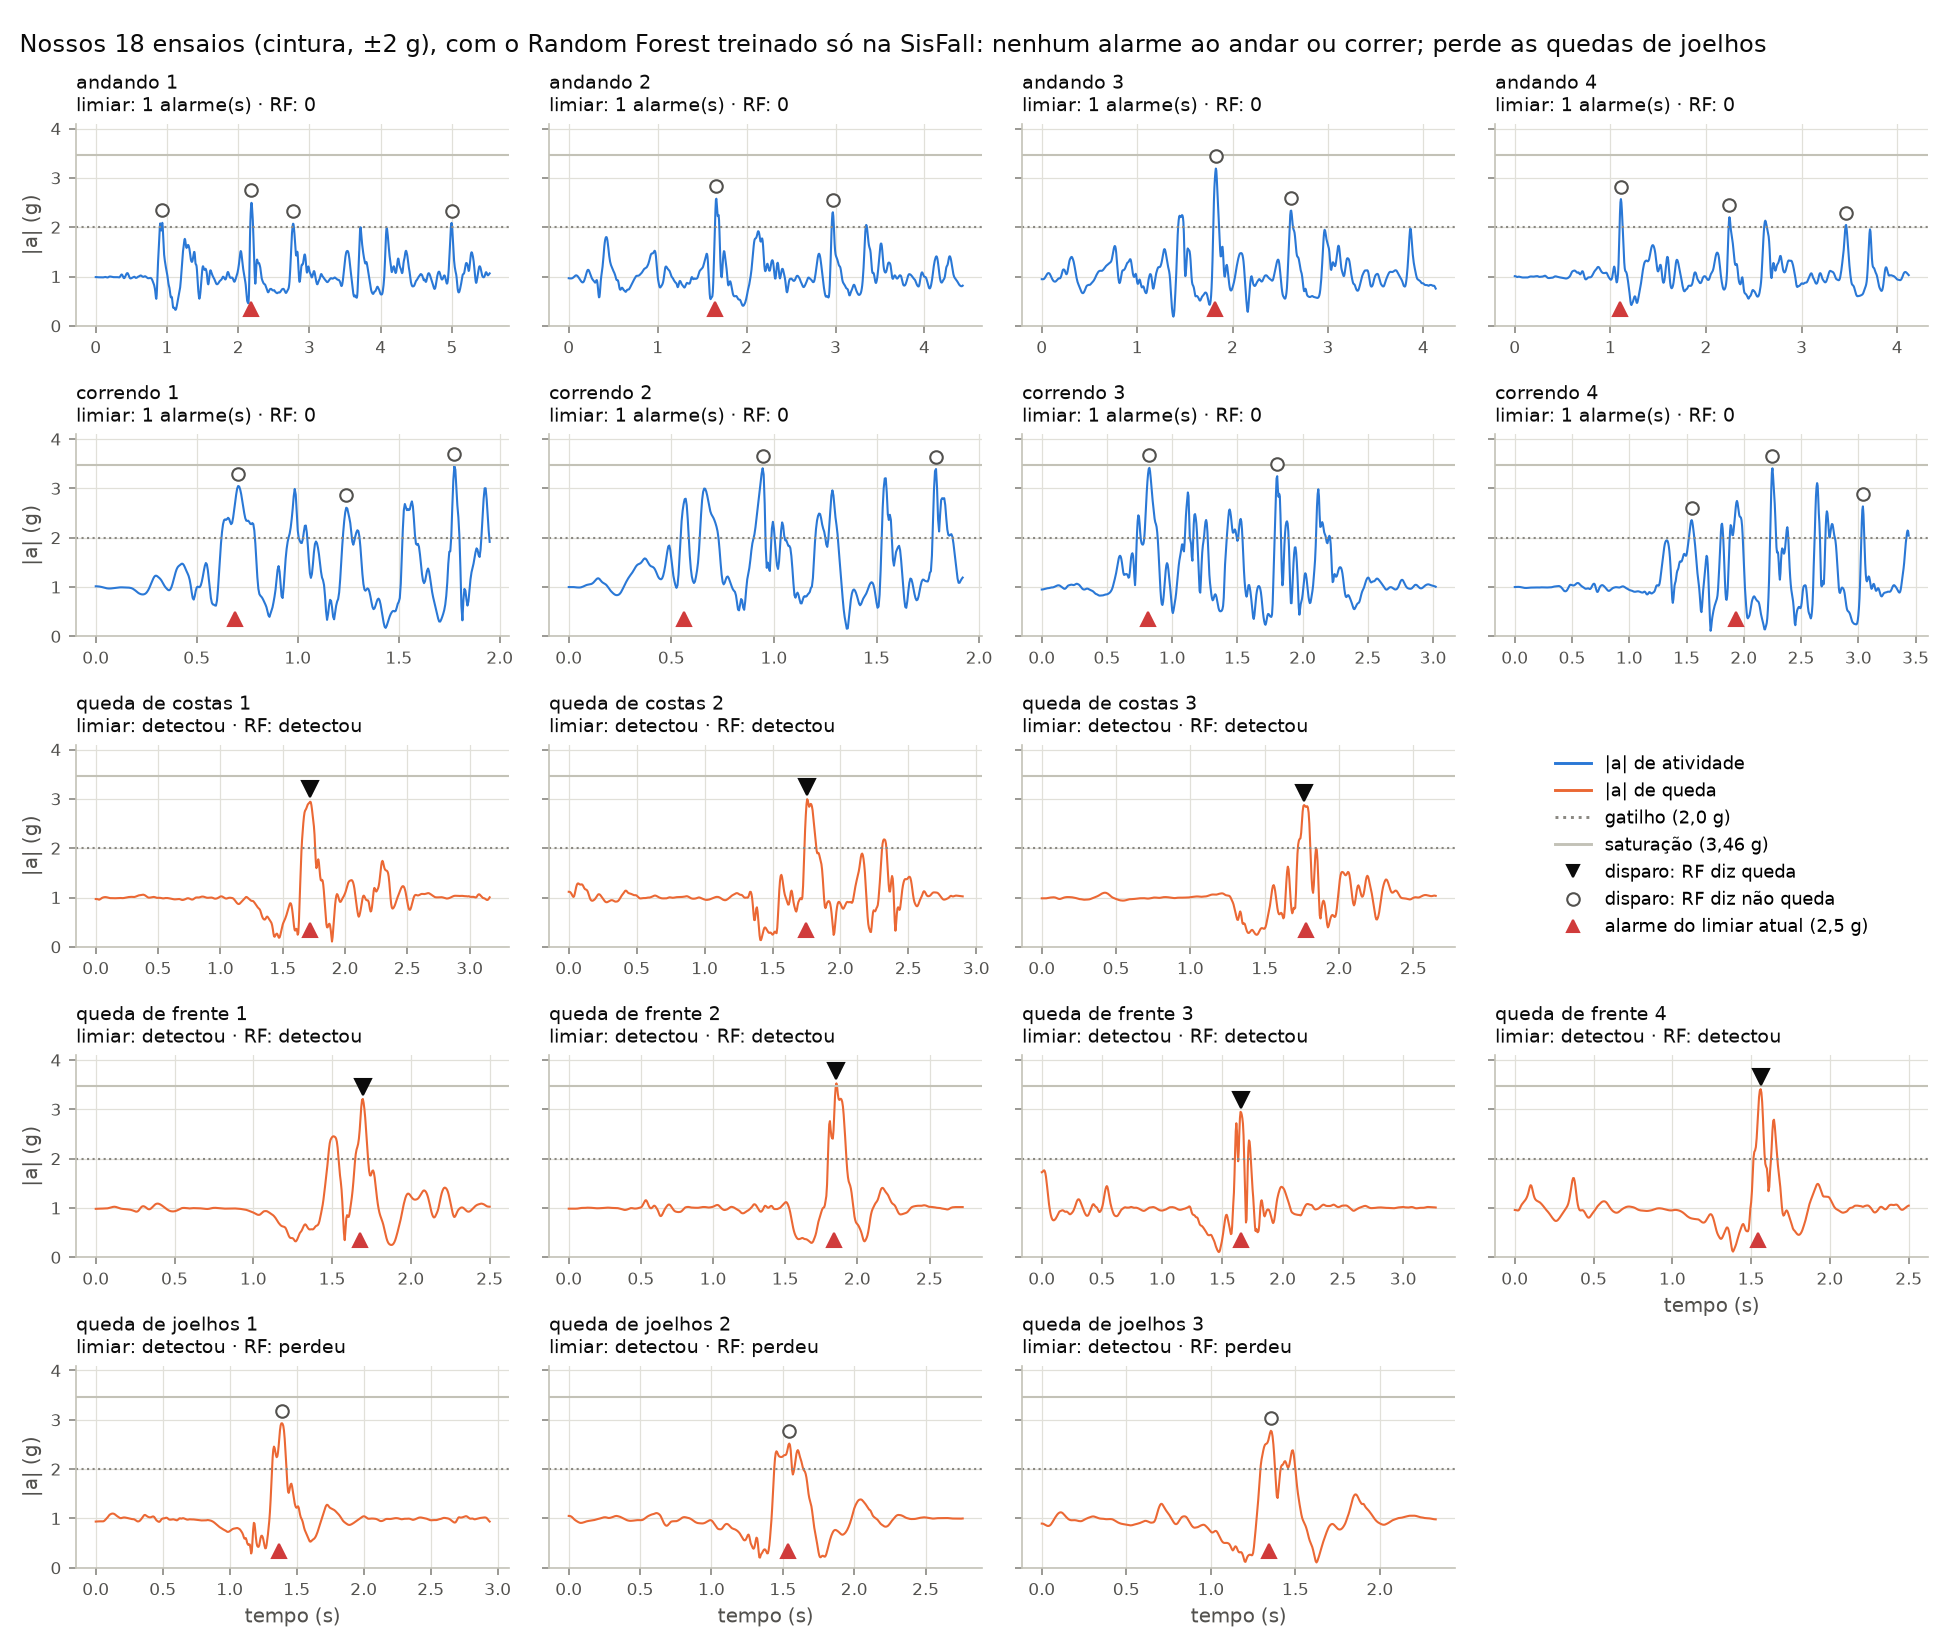
\includegraphics[width=\linewidth]{figuras/fig_proprios_ensaios.png}
\caption{Os 18 ensaios do primeiro semestre com o Random Forest treinado na SisFall.}
\label{fig:proprios}
\end{figure}

O modelo é \textbf{provisório}. Os dados de treino têm o sensor na cintura, e a pulseira vai no
pulso, onde o braço se move muito mais e o impacto chega diferente. O próximo passo é a coleta
no pulso, com várias pessoas e com o firmware atual ($\pm$8\,g), seguindo o protocolo de coleta
do projeto: os ensaios gravados pelo modo de coleta entram direto no treino, e o mesmo script
gera o novo modelo e os novos vetores de teste. Com esses dados, também vale reavaliar os
atributos de frequência, que na cintura melhoraram o resultado mas exigiriam uma FFT no
firmware.
